\chapter{Introduction}

%What does manifacturing mean?
\begin{quotation}
    \noindent
    \textsf{\textit{Manifacturing} is a word which is derived from Latin and it means \textit{made by hand}. This is suited to a reality where most commercial goods where totally made by hand. After many years, factory appeared and the way the products were made changed a lot! In particular the attention was on the use of \textit{machines} instead of \textit{handcrafted mehtods}. In the modern era machines, people and processes to handle them are grouped in complex \textit{production systems} that not rarely are \textbf{automated} and \textbf{computerized}.  
    }
\end{quotation}

\section{Production systems}
A \textbf{production system} is a compound of people, machine, procedures whose aim is to \textit{perform the manifacturing operations} of a firm. Any production system can be divided in two basic components: 
\begin{description}
    \itemsep-0.2em
    \item[\textsc{Facilities}] they consist of the factory (physical structure), machines, material handling and inspection equipments and all computer systems to control the manifacturing operations. The \textbf{plant layout} is included in this part and is related to the way equipment and workers are \textit{arranged} into the factory. Machines and general equipment are divide into \textbf{manifacturing systems} that are groups of machines to carry out some operations fort the production. Roughly speaking, they are all the components that "touch" the products.
    \item[\textsc{Manifacturing support systems}]  These are all the procedure used by the company to manage production and to solve all the problems related to it. In this branch are included product design, the planning of the manifacturing and some control and business operations.
\end{description}
\noindent
The  \Cref{fig:prod_sys_structure} shows schematically what we have just briefly explained here. Along this notes the scheme will be gradually enriched by other topics. 

\begin{figure}
    \centering
    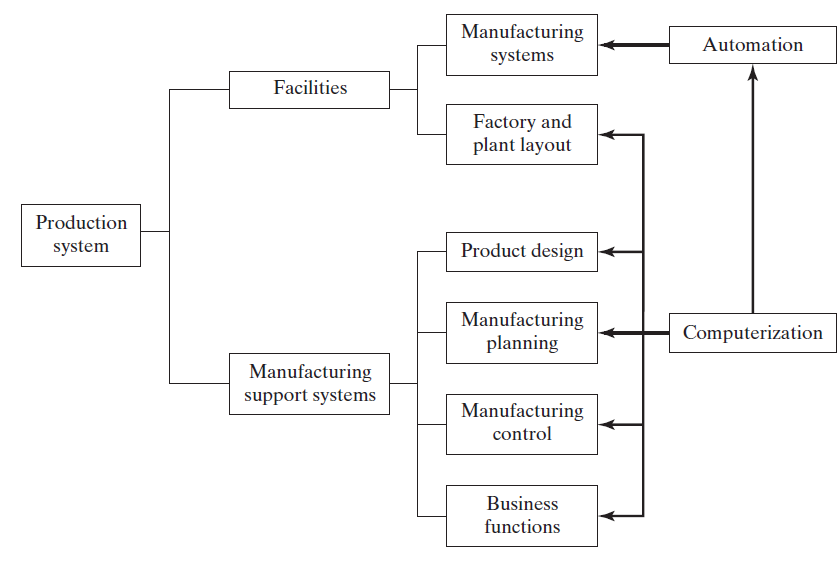
\includegraphics[scale=0.8]{img/prod_system_scheme.png}
    \caption{Production system structure and types of automation}
    \label{fig:prod_sys_structure}
\end{figure}

\section{Automation in production systems}
\textbf{Automation} refers to the possibility to substitute human through machines in order to execute different works. Mainly two types of automation on machines can be considered: (i) \textit{semiautomated machine} which execute only a part of the task independently; (ii) \textit{fully automated machine} is capable to work for long period without the human attention.\\
Some components of the production system are prone to be automated while other tasks require to operated manually. Also in these case we can divide such components in two categories:
\begin{enumerate}
    \itemsep-0.3em
    \item \textsf{\textbf{Automation} of the manifacturing systems}
    \item \textsf{\textbf{Computerization} of the manifacturing support systems}
\end{enumerate}

\subsection{Automated manifacturing systems}
Three basic types of automation can be distinguished that practically operates as fully automated systems.
\subsubsection{Fixed automation}
The sequence of processing operation is \textit{fixed} in the equipment configuration. If there is a sequence of operations to be performed they are usually simple, or they are combination of simple tasks. Such type of systems are used when there is the necessity to produce large quantities of pieces. They are suitable especially when there is small variations in the products.
\subsubsection{Programmable automation}
At the opposite, we find the \textbf{programmable automation}. Here there is the possibility to change the sequence of operations. The sequence of operations is dictated by a \textbf{program} which is a sequence of instructions written so that they can be interpreted by the system. They are used for low quantities and for batch production. Note that to produce a new batch of a different item: (i) we have to rewrite the program; (ii) we have to change the setup for equipments. This requires a \textit{changeover time}. Instances of programmable automation are Numerical controlled (NC) machines and Programmable logical controllers (PLCs).

\subsubsection{Flexible automation}
Such a type of automation is an extension of the previous with the difference that the changeover time is virtually avoided. What makes \textit{flexibility} possible is the fact that the differences between processed parts are not significant, so the changeover necessity is "little". Manifacturing systems which performs machinery processes are in this category.

\subsection{Computerized manifacturing support systems}
Automating the part of the production system devoted to manifacturing support is in order to reduce the manual and clerical required effort. In this context the term \textbf{Computer Integrated Manifacturing (CIM)} refers to the pervasive use of computers to \textit{design products}, \textit{plan the production}, \textit{control the operations} and so on. Other terms are used to indicate components of the CIM, in particular the \textit{Computer Aided Design (CAD)} supports the the design of the product, while \textit{Computer-Aided manifacturing (CAM)} is used for functions related to the planning.\\

A core operation in automation is \textbf{control}, which can be practically carried out using an \textbf{open-loop procedure} (or \textit{feedforward}) or in a \textbf{closed-loop} fashion, which exploting the negative feedback principle makes the overall system capable to correct the actions to be performed. Such a type of control strategy is used in the great majority of the application, this is why we focus on automation system which are based on them.

\subsection{Closed-loop automation system}
A \textbf{closed-loop automation system} can be divided into three subsystems: (i) Instrumentation subsystem, (ii) Control subsystem, (iii) Human-interface subsystem.

\begin{figure}[h]
    \centering
    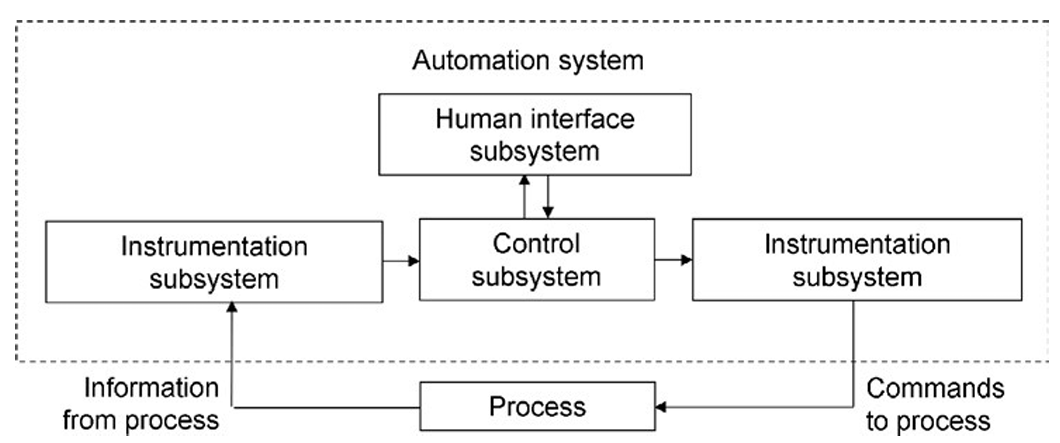
\includegraphics[scale=0.5]{img/closed_loop_automation.png}
\end{figure}

\subsubsection{i) Instrumentation subsystem}
Is the part devoted to the acquirement of information related to the behaviour of the process (by measuring its variables), such measurements are then sent to a conditioning circuit and then to the control subsystem. \\ 
The instrumentation devices (practically \textbf{sensors}) have different structures according to the input and output signals to be measured. They can be both analog or digital. Moreover they can be classified as \textbf{transducer} if their output is sent over short distances, \textbf{transmitter} if the output signal is sent over long distances.

\subsubsection{ii) Control subsystem}
It is the heart of any closed-loop automated system and it is in charge for carrying out several (basic) functions regarding: 
\begin{itemize}
    \itemsep-0.3em
    \item \textsf{Instrumentation subsystem}, in particular measured variables are compared to reference values in order to steer the control action through a certain direction by using again the instrumentation; 
    \item \textsf{Human Interface subsystem}, in particular the associated information are an input of the control part which through the instrumentation sends information to the process.
\end{itemize}


\subsubsection{iii) Human-Interface subsystem}

\subsubsection{How computers are involved in control}


\section{Levels of automation}